\Chapter{PRELIMINARY RESULTS}\label{sec:preliminary}\selectlanguage{english}

In this chapter, we present the preliminary results of this research work. These results are focused on the implementation of a probabilistically analysable instruction and data cache for the Ion MIPS32 processor on
FPGA. We developed a random placement and replacement policy that fulfills
all the requirements for PTA. Our experiments show that the cache fulfills all the requirements for PTA, and program timing can be determined with arbitrary accuracy. In addition, random placement and replacement improve the observed WCET from 6\% to 19\% w.r.t. a Least Recently Used policy.



\section{Relative Sensitivity Based Emulation}

This paper presents an FPGA implementation of a probabilistically analyzable
cache inspired by the simulation work presented
in~\cite{Kosmidis:2013:CDP:2485288.2485416}. In this paper we have
kept the same approach for the cache behaviour:
\begin{enumerate}
\item The cache uses a random replacement policy
\item The cache uses a parametric random placement policy based on
 a hash function
\item The cache placement is deterministic for each benchmark execution, but
  randomized across executions
\item We measure end-to-end execution time for a series of benchmarks
\end{enumerate}

\section{High-Level Fault Model}
\section{Sequential Circuits Fault model}
%\section{Hardware Implementation}
\label{Hardware Implementation}

%\subsection{Cache RTL Model}
\label{Cache Model}

We implemented an instruction and data cache for the Ion
MIPS32 processor~\cite{ION}. A completely novel, configurable cache
design was implemented in VHDL and integrated with the Ion core. The
cache is completely configurable (bus width, size, block size,
policies, etc.) with VHDL generics and could be easily ported to other
processor designs. Figure~\ref{fig:cache-structure} shows the main components of our design:

\begin{figure}
 \centering
  \captionsetup{justification=centering}    
   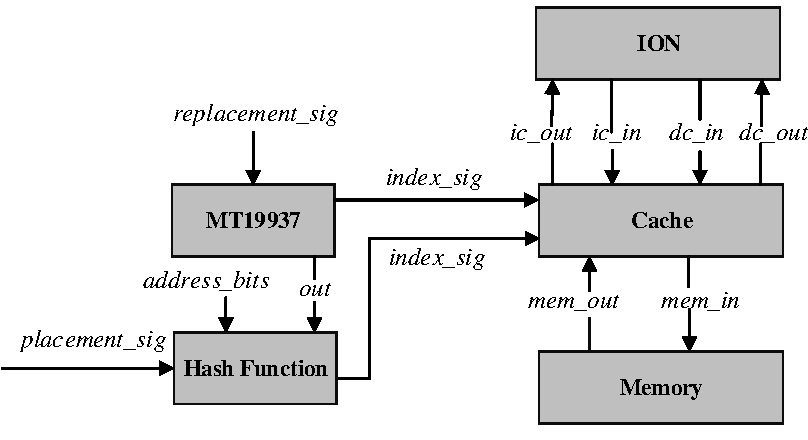
\includegraphics[scale=0.2]{figures/img/cache_structure_c.pdf}
   \caption{Structure of the proposed cache.}
\label{fig:cache-structure}
\end{figure}

\begin{enumerate}
\item The cache block contains the cache memory proper, as well as the
logic to manage the replacement policy (random and least-recently-used)
\item A hash function block that operates on the index signal to the
  cache, randomizing the mapping between memory blocks and cache blocks
\item A pseudo-random number generator (MT19937)
\item The Ion core, which provides a MIPS32 ISA and controls the whole
  system
\end{enumerate}

Our cache has three fundamentally novel features that enable probabilistic
timing analysis:
\begin{enumerate}
\item A random \textbf{placement} policy which uses a parametric hash
  function to shuffle the initial placement of blocks in the cache memory
\item A random \textbf{replacement} policy that uses high-quality random
numbers to provide statistically-verifiable guarantees that replacement
events are uniformly distributed among the available cache blocks
\item A high-quality pseudo-random number generation, with an extremely
long period, to generate random bits for the implementation of the cache
random policies
\end{enumerate}
%
%
%\subsection{Random Number Generation}

In our cache design, we used the Mersenne Twister algorithm to
generate random numbers. In particular, we used the MT19937 algorithm,
which is considered as a good hardware solution for a random number
generation~\cite{Matsumoto:1998:MTE:272991.272995}. MT19937 provides a
uniform pseudo number pattern with a period of
$2\textsuperscript{19937-1}$, with a width of 32 or 54 bits.  We used
the OpenCores implementation of MT19937~\cite{OpenCores}. The
synthesis report shows that the maximum clock frequency the design can
achieved is 147.016 MHz, with a throughput of 30 Msamples per second.

%\subsection{Parametric Hash Function}
%\label{PHF}
%
%The idea of using a parametric hash function for the implementation of
%random placement was given
%by~\cite{Kosmidis:2013:CDP:2485288.2485416}. This design is remodelled
%for this work, replacing their Multiply With Carry (MWC) random number
%generator with the MT19937, increasing the quality of the random
%numbers as well as the period.  The redesign was driven by the fact
%that MWC does not pass some statistical normality
%tests~\cite{bandyopadhyay2015discrete}, and its period might be
%insufficient for long running
%applications~\cite{Goresky:2003:EMR:945511.945514}.
%
%Standard placement assigns sets to cache lines based on the index bits
%of the memory address. If the placement policy assigns two memory
%addresses to the same cache set, they will systematically be in conflict. 
%To deal with this deterministic nature while randomizing the timing
%behaviour of the placement policy, we use a parametric hash
%function with a random number as an input.  A random number
%provides a unique and constant cache set mapping for each address.
%If the random number changes, the cache set in which the address is mapped changes. By changing random number only at a new execution, programs can be analyzed with end-to-end runs assuming that the cache is initially empty.
%Figure~\ref{fig:hash_function} shows the structure of the hash function.
%
%








%\subsection{Random Number Generation}
%
%In our cache design, we used the Mersenne Twister algorithm to
%generate random numbers. In particular, we used the MT19937 algorithm,
%which is considered as a good hardware solution for a random number
%generation~\cite{Matsumoto:1998:MTE:272991.272995}. MT19937 provides a
%uniform pseudo number pattern with a period of
%$2\textsuperscript{19937-1}$, with a width of 32 or 54 bits.  We used
%the OpenCores implementation of MT19937~\cite{OpenCores}. The
%synthesis report shows that the maximum clock frequency the design can
%achieved is 147.016 MHz, with a throughput of 30 Msamples per second.

%\subsection{Parametric Hash Function}
\label{PHF}


\begin{figure}[t!]

 \centering
  \captionsetup{justification=centering}    
   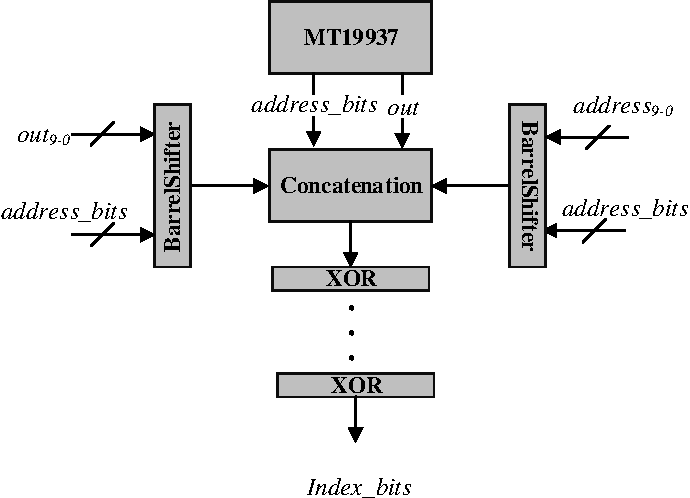
\includegraphics[scale=0.8]{figures/img/hash_function.pdf}
   \caption{The hash function uses a random number, the address bits, and four XOR stages to produce a random placement.}
\label{fig:hash_function}
\end{figure}



%\begin{figure}[t!]
%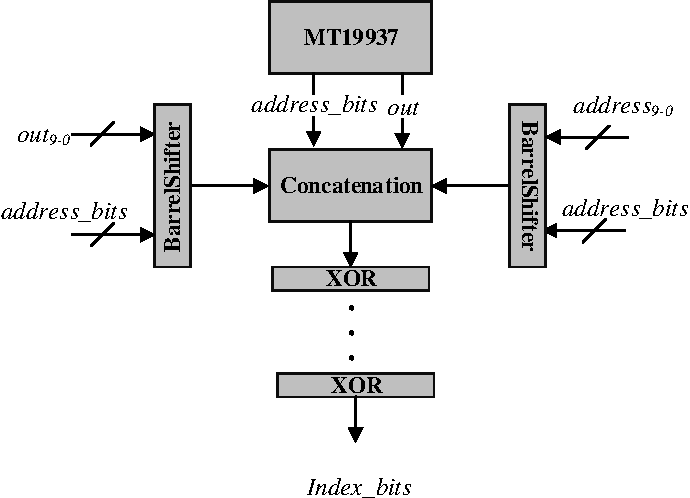
\includegraphics[width=\columnwidth]{figures/img/hash_function.pdf}
%\caption{The hash function uses a random number,
%the address bits, and four XOR stages to produce a random placement}
%\label{fig:hash_function}
%\end{figure}

The idea of using a parametric hash function for the implementation of
random placement was given
by~\cite{Kosmidis:2013:CDP:2485288.2485416}. This design is remodelled
for this work, replacing their Multiply With Carry (MWC) random number
generator with the MT19937, increasing the quality of the random
numbers as well as the period.  The redesign was driven by the fact
that MWC does not pass some statistical normality
tests~\cite{bandyopadhyay2015discrete}, and its period might be
insufficient for long running
applications~\cite{Goresky:2003:EMR:945511.945514}.

Standard placement assigns sets to cache lines based on the index bits
of the memory address. If the placement policy assigns two memory
addresses to the same cache set, they will systematically be in conflict. 
To deal with this deterministic nature while randomizing the timing
behaviour of the placement policy, we use a parametric hash
function with a random number as an input.  A random number
provides a unique and constant cache set mapping for each address.
If the random number changes, the cache set in which the address is mapped changes. By changing random number only at a new execution, programs can be analyzed with end-to-end runs assuming that the cache is initially empty.
Figure~\ref{fig:hash_function} shows the structure of the hash function.






%



%\section{Experimental Results}

\begin{table}[t]
\caption{Resource utilization and overhead (Virtex-5)}
\label{resource_table}
\begin{center}
\begin{tabular}{llllll}
\toprule
              & LRU & \multicolumn{3}{c}{RND} & Overhead \\
\cmidrule(lr){3-5}
              &   &  Cache & Hash	& MT19937 &  \\
\midrule
%Available     & 69120    &       69120   & 69120           \\
LUT Flip Flop  & 1904    &  1792   &  656   &  117  & 34.7\% \\ 
Slice LUTs     & 6026    &  5637   &  660   &  419  & 11.6\%  \\
%BRAMs          & 4       &  6      &  2     &  1    & 225\%\\
\bottomrule
\end{tabular}
\end{center}
\end{table}


\begin{figure}[t!]

 \centering
  \captionsetup{justification=centering}    
   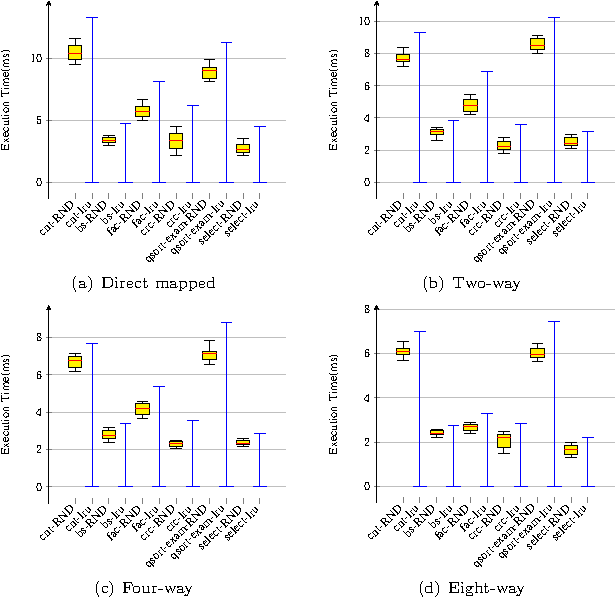
\includegraphics[scale=0.8]{figures/img/boxplot.pdf}
   \caption{Execution Time Measurement}
\label{fig:boxplot}
\end{figure}
The architecture used in our experiments is the OpenCores Ion MIPS32
processor. We integrated both an I-cache and a D-cache, and we
implemented the whole system on the Xilinx ML505 FPGA evaluation
board, using the XC5VLX110T chip using  Xilinx ISE-14.4 and ModelSim 10.1.a. We used two separate 4~kB cache
memories for data and instructions, both with a 32-byte line size.  To
evaluate our design, we used M\"alardalen real-time benchmark~\cite{mrtc:bench} suite. We selected six benchmarks: \textit{cnt, bs,
  fac, crc, qsort-exam and select}. These benchmarks use arrays
and matrices, and have nested loops structures which are ideal to test
our design~\cite{Competitive}. We omitted those benchmarks using
external libraries and unstructured code to simplify the
software implementation and data collection. 



Each benchmark was run on multiple cache configurations profiles, and
we derived its execution time profile using MBPTA, with 30 runs per
profile to approximate a normal error distribution.
To show that our cache generates identically distributed execution times (as
required for PTA), we used the Kolmogorov-Smirnov test~\cite{books/daglib/0020904},
which shows that the null hypothesis (the data are normally distributed) cannot
be rejected for all benchmarks at the 5\% confidence level ($p>0.062$).
We compared our results (RND) with a standard Least-Recently-Used (LRU)
cache policy implementation.

Figures \ref{fig:boxplot} show the timing
distributions for all benchmarks on our cache from direct-mapped to
8-way associative, respectively. As an added advantage, our random
cache shows a 19\% improvement in worst case execution time w.r.t to
LRU for a direct-mapped cache, 11\% for 2-way cache, 8\% for a 4-way
cache, and 6\% for an 8-way cache. As expected, LRU gets closer to RND
as the number of ways increases: the number of conflict miss is
greatly reduced by additional ways.

\section{Conclusion}
In this paper, we present the RTL model of a randomized L1 data and
instruction cache. This cache uses a high-quality random number
generator for random placement and replacement. Random placement is
obtained with a parametric hash function that shuffles the association
between memory addresses and cache blocks. The cache is integrated
with the Ion MIPS32 processor, and verified to generate independent
and identically distributed timing events, such that Measurement-Based
Probabilistic Timing Analysis is possible (MBPTA). We test our cache
and MBPTA approach on a variety of benchmark from the M\"alardalen
benchmark suite and show a noticeable improvement (5-15\%) in terms of
measured Worst Case Execution Time (WCET) as well as enabling the
identification of safe probabilistic WCET (pWCET) bounds.  Future work
will consider the implementation of shared randomized caches for
multi-core architectures.
